%----------------------------------------
% Write your notes here
%----------------------------------------

\section{Random Assignments}
\subsection{Definition}
\textbf{Random Assignment} is an experimental technique for assigning participants to different groups in an experiment using randomization.
\subsection{Example: Neyman's Model}
Random assignment breaks the link between the confounds and the results. The following example discusses the details of random assignment using Neyman's Model, and provides ground for understanding instrumental variables (section 2.2).
\\
\\
In the experiment, each person is represented by a ticket, $T_i$$|$$C_i$. $T_i$ represents the outcome under treatment, and $C_i$ represents the outcome under control. By randomly picking participants into treatment/control group, we want to observe the average treatment effect, $ATE$, by calculating the outcome differences. In each group, we only observe the corresponding outcome.

\begin{figure}[ht]
  \begin{center}
    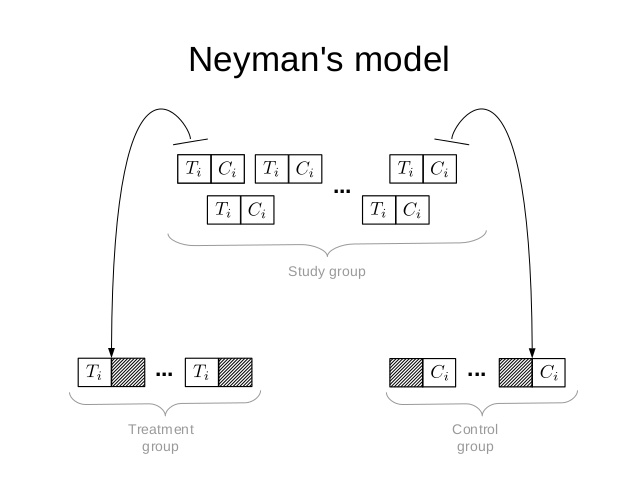
\includegraphics[width=0.5\textwidth]{figures/natural-experiments-31-638.jpg}
    \caption{Neyman's Model
      }
    \label{fig:Neyman's Model}
  \end{center}
\end{figure}

Since the sample is randomly selected, the average of the sample is an unbiased estimator of the true average. 

\begin{itemize}
\item Average treatment outcome: $\hat{\overline{T}} = \frac{1}{N}\sum{T_i}$
\item Average control outcome: $\hat{\overline{C}} = \frac{1}{N}\sum{C_i}$
\item Average treatment effect: $\hat{\overline{ATE}} = \hat{\overline{T}} - \hat{\overline{C}}$
\end{itemize}

\subsection{Problems of Random Assignment}
Random Assignment does have several problems:
\begin{itemize}
\item \textbf{Small sample sizes}: When the sample size is small, the experiment is subject to statistical variation. Denote $\alpha$ to be the significance level, and power, $(1-\beta)$, to be the chance of detecting a real effect if the effect exists. In the following figure, $\alpha$ is 5\%, and $(1-\beta)$ is 35\%. Assume that 30\% of the investigated effects are real, the false discovery rate is 25\%. 
\begin{figure}[ht]
  \begin{center}
    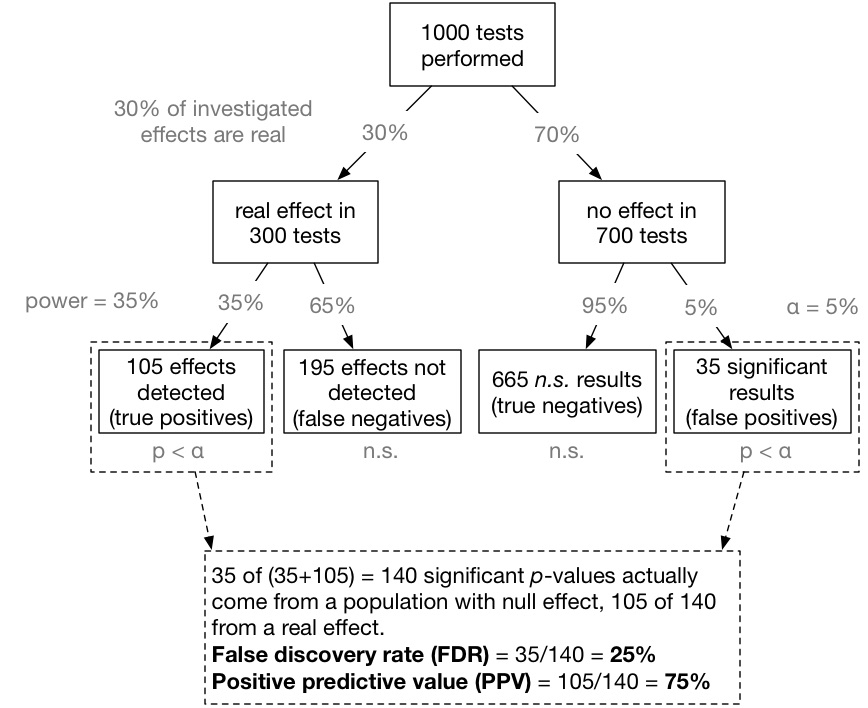
\includegraphics[width=0.5\textwidth]{figures/PPV_tree.jpeg}
    \caption{Small Sample
      }
    \label{fig:Small Sample}
  \end{center}
\end{figure}
\\
Small sample sizes is commonly seen in many experiments today in social sciences. A good counter measure to it is to run a pilot study along with a power proportion test to discover the sample size needed. Usually, the lower the rate of real investigated effects is, the higher the sample size should be.
\item \textbf{Researchers' degree of freedom, Publication Bias, p-hacking}: The variation of researchers' choice to run different tests or choose different sets of data is sometimes even larger than the variation in the data or experiment.
\end{itemize}

\section{Natural Experiments}
\subsection{Definition}
\textbf{Natural Experiment} is an empirical study in which individuals (or clusters of individuals) exposed to the experimental and control conditions are determined by nature or by other factors outside the control of the investigators, but the process governing the exposures arguably resembles random assignment.

\subsection{Instrumental Variables}
An instrumental variable in natural experiments is independent of the confounds and changes the distribution in the results. In the case of studying the correlation of military service and future earnings, the lottery of assigning military service is the instrumental variable. However, the assignment is different from the actual, and we need to consider the case of non-compliance.
\\
\begin{figure}[ht]
  \begin{center}
    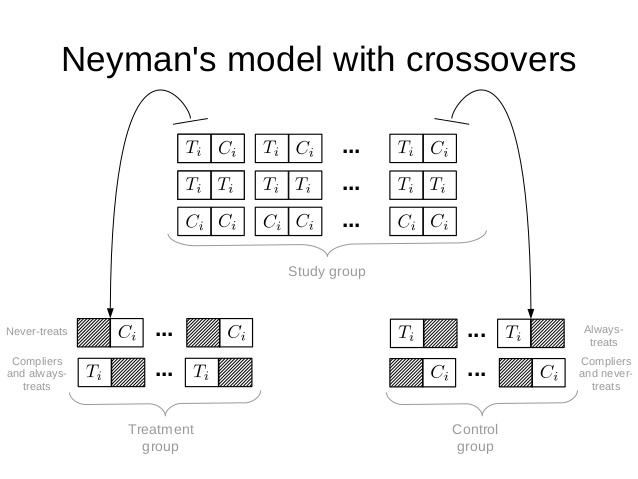
\includegraphics[width=0.5\textwidth]{figures/natural-experiments-37-638.jpg}
    \caption{Non-compliance
      }
    \label{fig:Non-compliance}
  \end{center}
\end{figure}
\\
Figure 3 shows the case of non-compliance in the previous treatment example. Consider the following three types of people: (a) Compliers, who complies to the given assignment (b) Always-treats, who always receive treatment regardless of the assignment (c) Never-treats, who always do not receive treatment.
\\
\\
Denote $ATE_c$, $ATE_a$, $ATE_n$ to be the average treatment effect of the groups (a),(b) and (c), $p_c$, $p_a$, $p_n$ to be the proportion of the three groups in the sample. Since group (b) and (c) will show no different in effect regardless of their assignments, the $ATE$ for these groups are 0. Therefore, we have: $\hat{\overline{ATE}} = \hat{\overline{ATE_c}}p_c$. Note that the number we care about is $ATE_c$.
\\
\\
To estimate $p_c$, we can observe the rate of accepting assignment in treatment and control group and get the proportion by subtraction.
\subsection{Regression Discontinuities}
Sometimes in experiments, an arbitrary threshold would have an effect in the regression output. 
\\
\\
In class we are given an example of Yelp rating. The rounded value of rating presented to users caused a jump in regression result around the rounding threshold.





